% Provenance (never printed): see sources/outline_sources.md (Year 2: monsoons; El Niño--Southern
% Oscillation; the North Atlantic Oscillation; ocean--atmosphere coupling). Definitions after the
% IPCC AR6 glossary, the NOAA CPC ENSO FAQ and NAO pages, the NWS glossary and the IMD monsoon
% FAQ; indices from the CPC data files (data/derived/bachelor-2-{oni,oni-table,roni,nino34,nao});
% figures from figdata/bachelor-2/climvar.py; values of the examples, exercises and problem
% computed in the Book 4 scratch calculator calc/ch23.py.
\chapter{Variabilidade climática}\label{ch:b2:climate-variability}

Em setembro de 2026 a superfície do mar no Pacífico equatorial central teve uma média de \qty{29.27}{\celsius},
onde o valor habitual de setembro é \qty{26.71}{\celsius}; mais a leste, partes do oceano estavam
mais de \qty{4}{\celsius} acima do habitual, e os previsores davam mais de quatro chances em cinco
de o evento, até o fim do ano, ultrapassar todos os El~Niño desde 1950. Os eventos
recordes anteriores, em 1982, 1997 e 2015, branquearam e mataram corais, incendiaram florestas tropicais
e trouxeram ondas de calor; a captura de anchoveta do Peru cai fortemente quando essa água quente persiste. O
oceano e a atmosfera do Pacífico tropical tinham oscilado, como fazem a cada poucos anos, e a
oscilação chegou muito além do Pacífico. Este
capítulo descreve essas oscilações do clima, as \omterm{def:b2:climate-variability:monsoon}{monções}, o El~Niño e a La~Niña, a \omterm{def:b2:climate-variability:nao}{Oscilação do
Atlântico Norte}, e o que faz do oceano sua memória.
% ledger: data:b4-nino34, cpc:edd-2026-10, thirumalai24:bjerknes, cheung26:peru

\begin{recall}
\textbf{Dos volumes escolares}: tempo e clima; a anomalia de temperatura; a camada de mistura,
a termoclina e a ressurgência; a retroalimentação climática. \textbf{Do volume do primeiro ano}: as células
de Hadley, os ventos alísios, a zona de convergência intertropical e sua migração sazonal, a circulação
de Walker, a ressurgência costeira. \textbf{Do \cref{ch:b2:weather-systems}}: a corrente de jato,
as \omterm{def:b2:weather-systems:rossby}{ondas de Rossby}, os ciclones extratropicais e o bloqueio. \textbf{Dos livros de física}: a capacidade térmica
e o primeiro princípio da termodinâmica.
\end{recall}

\section{A variabilidade e suas medidas}\label{sec:b2:climate-variability:measures}

O tempo muda de um dia para o outro; o clima, a estatística do tempo, também muda, de uma estação
ou de um ano para o seguinte, mesmo quando nada fora do sistema climático muda. Parte dessa
variabilidade é ruído, mas grande parte organiza-se em alguns padrões que se repetem, com sua própria
geografia e suas próprias escalas de tempo.

\begin{definition}[Modo de variabilidade climática; índice climático; climatologia]\label{def:b2:climate-variability:modes}
Um \emph{modo de variabilidade climática}\index{modo de variabilidade climática} é um padrão recorrente de
variabilidade natural do sistema climático, com sua própria estrutura espacial, sazonalidade e escalas
de tempo, que nasce da dinâmica da atmosfera ou do acoplamento entre o oceano e a
atmosfera. Um \emph{índice climático}\index{índice climático} é uma série temporal construída a partir de variáveis
climáticas que resume o estado de um tal padrão, por exemplo a diferença de pressão ao nível do mar
entre a Islândia e os Açores. A \emph{climatologia}\index{climatologia} de uma variável
é sua média sobre um período de referência, calculada para cada mês ou estação do calendário; o período
de referência padrão tem 30 anos, atualmente 1991--2020.
\end{definition}
% ledger: ipccgl:modes, ipccgl:index, wmo:normal-30yr

Muitos modos são movidos por processos internos ao sistema climático: fazem parte de sua
variabilidade interna. Como se repetem com suas próprias escalas de tempo, são uma fonte de
previsibilidade fora do alcance das previsões do tempo, de semanas a décadas. Os índices tornam-nos
mensuráveis. Um índice é calculado a partir de anomalias, como nos volumes escolares, e
suavizado.
% ledger: ipccgl:modes

\begin{method}[Das observações a um índice]\label{met:b2:climate-variability:index}
\begin{enumerate}
  \item Calcule-se a \omterm{def:b2:climate-variability:modes}{climatologia}: a média da variável para cada mês do calendário ao longo do
        período de referência.
  \item Subtraia-se: a anomalia de cada mês é seu valor menos a \omterm{def:b2:climate-variability:modes}{climatologia} desse mês.
        O ciclo sazonal desaparece; o que resta é a variabilidade.
  \item Suavizem-se as anomalias com uma média móvel, a média de $n$ valores consecutivos centrada em
        cada mês, para eliminar as flutuações mais curtas que o padrão de interesse.
  \item Se o índice for comparado com outros, divida-se por seu desvio-padrão: o índice
        fica então padronizado, em unidades de desvio-padrão.
\end{enumerate}
\end{method}

\begin{example}[Uma anomalia]\label{ex:b2:climate-variability:anomaly}
A temperatura média da superfície do mar do Pacífico equatorial central entre \ang{5} N e
\ang{5} S, \ang{170} W e \ang{120} W foi de \qty{29.27}{\celsius} em setembro de 2026. Sua \omterm{def:b2:climate-variability:modes}{climatologia}
de setembro é \qty{26.71}{\celsius}, logo a anomalia foi de $29.27 - 26.71 = \qty{2.56}{\celsius}$.
Em setembro de 1997 o mesmo oceano estava a \qty{28.79}{\celsius} contra \qty{26.73}{\celsius}, uma
anomalia de \qty{2.06}{\celsius}. As duas \omterm{def:b2:climate-variability:modes}{climatologias} diferem ligeiramente porque o período de
referência é deslocado a cada cinco anos: o próprio oceano aqueceu.
% ledger: data:b4-nino34, cpc:oni-def
\end{example}

\section{Monções}\label{sec:b2:climate-variability:monsoons}

\begin{definition}[Monção]\label{def:b2:climate-variability:monsoon}
Uma \emph{monção}\index{monção} é um vento de origem térmica, nascido do aquecimento desigual de
uma massa continental e do oceano vizinho, que inverte seu sentido com as estações, junto com
a inversão sazonal das chuvas que ele traz.
\end{definition}
% ledger: nws4:monsoon, ipccgl:monsoon

Em terra o calor do Sol de verão fica numa camada fina perto da superfície, enquanto o mar mistura
o mesmo calor para baixo em sua camada de mistura, com dezenas de metros de profundidade, e aquece muito menos. O ar sobre
a terra aquece mais, sua pressão à superfície cai, e o ar úmido vem do mar, sobe, esfria e
chove; em altitude o ar volta em direção ao mar. No inverno a terra é a superfície mais fria e a circulação
inverte-se. Tomadas em conjunto, as \omterm{def:b2:climate-variability:monsoon}{monções} do planeta formam um único padrão global que domina o ciclo
anual da chuva tropical e subtropical; seu domínio define-se como as regiões onde a chuva média
do verão local excede a do inverno em mais de \qty{2.5}{mm} por dia.
% ledger: nws4:monsoon, ipccgl:monsoon

\begin{omfigure}
\centering
\begin{tikzpicture}[font=\scriptsize, >=Stealth]
\foreach \col/\title in {0/{a\enspace verão}, 7.2/{b\enspace inverno}} {
  \begin{scope}[shift={(\col,0)}]
  \node[anchor=south west] at (0,3.0) {\textbf{\title}};
  \fill[ocBlue!18] (0,0) rectangle (3,0.35);
  \fill[brown!35] (3,0) -- (6.4,0) -- (6.4,0.5) -- (3,0.35) -- cycle;
  \node at (1.5,0.17) {mar};
  \node at (4.7,0.2) {terra};
  \end{scope}
}
% summer: low over the land, inflow from the sea, rising air and rain
\node[font=\small\bfseries, ocBlue] at (0.45,0.62) {H};
\node[font=\small\bfseries, ocRed] at (4.8,0.78) {L};
\node[ocRed, anchor=west] at (5.35,0.78) {quente};
\draw[->, thick] (1.0,0.98) -- (4.2,1.02);
\node at (2.4,0.66) {ar úmido vindo do mar};
\draw[->, thick] (4.8,1.15) -- (4.8,2.55);
\draw[->, thick] (4.45,2.8) -- (1.75,2.8);
\draw[->, thick] (1.4,2.6) -- (1.4,1.25);
\fill[black!15, draw=black!40] (4.0,1.9) .. controls (4.0,2.55) and (5.6,2.55) .. (5.6,1.9) -- cycle;
\foreach \x in {4.25,4.5,5.1,5.35} {\draw[ocBlue, dashed] (\x,1.85) -- (\x-0.1,1.2);}
\node[anchor=west] at (5.65,2.1) {chuva};
% winter: high over the land, dry outflow to the sea
\begin{scope}[shift={(7.2,0)}]
\node[font=\small\bfseries, ocRed] at (0.45,0.62) {L};
\node[font=\small\bfseries, ocBlue] at (4.8,0.78) {H};
\node[ocBlue, anchor=west] at (5.35,0.78) {frio};
\draw[->, thick] (4.2,1.02) -- (1.0,0.98);
\node at (2.4,0.66) {ar seco vindo da terra};
\draw[->, thick] (1.4,1.25) -- (1.4,2.6);
\draw[->, thick] (1.75,2.8) -- (4.45,2.8);
\draw[->, thick] (4.8,2.55) -- (4.8,1.15);
\end{scope}
\end{tikzpicture}
\par\smallskip{\small A \omterm{def:b2:climate-variability:monsoon}{monção} como circulação terra--mar (corte esquemático, fora de escala): no
verão a terra é a superfície mais quente, com baixa pressão junto ao solo, entrada de ar úmido vindo
do mar, ar ascendente e chuva; no inverno a circulação inverte-se e o vento de terra é seco.}
\end{omfigure}
% ledger: nws4:monsoon, imd:heat-low

A \omterm{def:b2:climate-variability:monsoon}{monção} do Sul e do Sudeste da Ásia começa no fim de maio ou no início de junho, progride
para nordeste e termina no fim de setembro ou no início de outubro. Antes dela, as terras em volta do
mar Arábico aquecem: em junho a superfície envia cerca de \qty{160}{W/m^2} de calor para o ar sobre
o noroeste árido da Índia, o Paquistão e o Oriente Médio, e forma-se ali uma baixa térmica pouco profunda,
que chega só a cerca de \qty{1.5}{km}, com pouca chuva; uma baixa térmica fraca, como no ano de seca
de 1987, significa uma atração fraca sobre o ar úmido do oceano. Dela parte um cavado alongado de baixa pressão, o cavado
da \omterm{def:b2:climate-variability:monsoon}{monção}, até o fundo do golfo de Bengala; suas oscilações norte--sul trazem os períodos
ativos e as pausas da estação. Sobre a Índia como um todo a chuva de junho a setembro tem média de
\qty{88}{cm}, com um desvio-padrão de \qty{9}{cm}, cerca de \qty{10}{\percent}: uma estação a menos de
\qty{10}{\percent} da média de longo período é chamada normal. Na costa de Kerala, onde o
serviço meteorológico nacional declara o início da \omterm{def:b2:climate-variability:monsoon}{monção} a partir da chuva de catorze estações,
dos ventos e da radiação infravermelha emitida medida por satélite, a chuva média é de
\qty{556}{mm} em junho e \qty{659}{mm} em julho.
% ledger: ipccgl:monsoon, imd:heat-low, imd:lpa, imd:onset

A \omterm{def:b2:climate-variability:monsoon}{monção} da África Ocidental traz ventos úmidos de sudoeste vindos do golfo da Guiné, progredindo
para o norte de maio a setembro; sua chuva atinge o máximo perto de \ang{12} N no fim de agosto e em setembro e
recua a partir de outubro.
% ledger: ipccgl:monsoon

Uma \omterm{def:b2:climate-variability:monsoon}{monção} é regular em seu calendário, irregular em sua quantidade, e as oscilações de um ano para outro do
Pacífico tropical estão entre as causas. Os anos de El~Niño tendem a deixar a Índia com falta de chuva: as
secas de 1904, 1972 e 1987 vieram com o El~Niño. A ligação não é certa: em 1997 um forte
El~Niño coincidiu com uma fase positiva do Dipolo do Oceano Índico, um modo visto mais adiante, e a Índia
teve uma \omterm{def:b2:climate-variability:monsoon}{monção} quase normal.
% ledger: narang24:enso-monsoon, ipccgl:other-modes

\section{El Niño e a Oscilação Sul}\label{sec:b2:climate-variability:enso}

O volume do primeiro ano descreveu a circulação de Walker: o ar que sobe sobre o Pacífico ocidental quente,
corre para leste em altitude, desce sobre o Pacífico oriental fresco e volta para oeste com os ventos
alísios. No oceano abaixo, os alísios acumulam a água quente no oeste, onde a termoclina é
profunda, e fazem subir água fria ao longo do equador no leste, onde ela é rasa. Esse estado não é
fixo.

\begin{definition}[El Niño--Oscilação Sul; El Niño; La Niña; Oscilação Sul]\label{def:b2:climate-variability:enso}
O \emph{El Niño--Oscilação Sul}\index{El Niño--Oscilação Sul} (ENSO) é o
modo acoplado oceano--atmosfera do Pacífico tropical: variações coerentes, de um ano para outro, da
temperatura da superfície do mar, da chuva convectiva, da pressão à superfície e da circulação ao longo
do Pacífico equatorial, com escalas de tempo preferenciais de dois a cerca de sete anos. O \emph{El
Niño}\index{El Niño} é sua fase quente, um aquecimento da superfície do mar do Pacífico equatorial central e
centro-oriental; a \emph{La Niña}\index{La Niña} é sua fase fria, um resfriamento da
mesma região. A \emph{Oscilação Sul}\index{Oscilação Sul} é sua parte atmosférica,
uma gangorra de pressão à superfície entre o Pacífico tropical ocidental e o oriental: durante o El~Niño
a pressão é mais alta que a média sobre a Indonésia e o Pacífico ocidental e mais baixa sobre o
Pacífico oriental, e o inverso durante a La~Niña.
\end{definition}
% ledger: cpc:enso-faq, cpc:enso-faq-so, ipccgl:enso

Durante o El~Niño, os alísios de leste enfraquecem ao longo do equador, e no oeste os
ventos de baixos níveis podem até soprar de oeste; a água quente do oeste espalha-se para leste, e a convecção
profunda e sua chuva a acompanham, deixando a Indonésia e o norte da Austrália mais secos. A superfície do mar
do Pacífico centro-oriental fica tipicamente \qtyrange{1.5}{2.5}{\celsius} acima da média, e
a termoclina ali fica a \qtyrange{150}{175}{m}, mais funda que o habitual. Durante a La~Niña os alísios
reforçam-se em toda a bacia, a superfície do mar fica \qtyrange{1}{2}{\celsius} abaixo da
média, e a termoclina no leste sobe para \qtyrange{50}{100}{m}. A circulação de Walker
enfraquece durante o El~Niño e reforça-se durante a La~Niña. Os episódios repetem-se tipicamente a cada três a
cinco anos, com intervalos que variaram de dois a sete; um El~Niño dura tipicamente nove a
doze meses, uma La~Niña de um a três anos. Ambos tendem a se desenvolver entre março e junho, a
atingir o máximo entre dezembro e abril e a enfraquecer entre maio e julho; seus efeitos são mais fortes
de dezembro a abril, quando a superfície do mar equatorial está mais quente.
% ledger: cpc:enso-faq-features, cpc:enso-faq-timing

\begin{omfigure}
\centering
\begin{tikzpicture}[font=\scriptsize, >=Stealth, x=1cm, y=0.8cm]
\foreach \row/\title/\tw/\te/\rx/\cwidth in {
    0/{a\enspace neutro}/1.15/0.35/1.6/1.0,
    -4.6/{b\enspace El Niño}/0.95/0.85/5.6/1.4,
    -9.2/{c\enspace La Niña}/1.3/0.18/1.0/0.8} {
  \begin{scope}[shift={(0,\row)}]
  \node[anchor=south west] at (0,2.55) {\textbf{\title}};
  % ocean: warm layer above the thermocline
  \fill[ocBlue!20] (0,-1.5) rectangle (11,0);
  \fill[omWarm!25] (0,0) -- (0,-\tw) .. controls (4,-\tw) and (7,-\te) .. (11,-\te) -- (11,0) -- cycle;
  \draw[thick, ocBlue!70!black] (0,-\tw) .. controls (4,-\tw) and (7,-\te) .. (11,-\te);
  \draw (0,0) -- (11,0);
  % convection and Walker cell
  \fill[black!15, draw=black!40] ({\rx-\cwidth/2},0.5) .. controls ({\rx-\cwidth/2},2.1) and ({\rx+\cwidth/2},2.1) .. ({\rx+\cwidth/2},0.5) -- cycle;
  \draw[->, thick] (\rx,0.55) -- (\rx,2.15);
  \draw[->, thick] ({\rx+0.4},2.3) -- (9.6,2.3);
  \draw[->, thick] (10.0,2.1) -- (10.0,0.5);
  \draw[->, thick] (9.6,0.3) -- ({\rx+0.7},0.3);
  \end{scope}
}
\node[anchor=west] at (2.3,1.4) {ar ascendente, chuva};
\node[anchor=east] at (9.9,1.4) {ar descendente};
\node at (6.0,0.55) {alísios};
\node[anchor=west, ocBlue!70!black] at (7.6,-0.95) {termoclina};
\node[anchor=east] at (4.8,-4.6+1.4) {a chuva vai para leste};
\node at (8.2,-4.6+0.55) {alísios fracos};
\node at (6.0,-9.2+0.55) {alísios fortes};
\node[ocBlue!70!black, align=center] at (9.6,-9.2-0.8) {água fria\\perto da superfície};
\node[anchor=north west] at (0,-9.2-1.55) {oeste (Indonésia)};
\node[anchor=north east] at (11,-9.2-1.55) {leste (América do Sul)};
\end{tikzpicture}
\par\smallskip{\small O Pacífico equatorial ao longo do equador nas três fases do ENSO
(esquemático, fora de escala): a circulação de Walker em cima, a camada superior quente e a
termoclina embaixo. Durante o El~Niño os alísios enfraquecem, a água quente e a chuva espalham-se para leste
e a termoclina no leste aprofunda-se até \qtyrange{150}{175}{m}; durante a La~Niña os alísios
reforçam-se e a termoclina no leste sobe para \qtyrange{50}{100}{m}.}
\end{omfigure}
% ledger: cpc:enso-faq-features, climategov:walker

Os nomes vêm de séculos diferentes e de ciências diferentes. Os pescadores da costa da
América do Sul notavam um aquecimento de suas águas costeiras por volta do Natal que perturbava a
pesca, e chamaram-no El~Niño, o menino. Sir Gilbert Walker descobriu a \omterm{def:b2:climate-variability:enso}{Oscilação
Sul} na atmosfera, sem ligá-la ao oceano. Só no fim dos anos 1960 Jacob Bjerknes e outros viram que os
dois eram um só fenômeno. Os termos La~Niña e neutro ganharam destaque nos anos 1980.
% ledger: climategov:enso-history, ipccgl:enso

\begin{history}[O menino dos pescadores]
\begin{minipage}[t]{0.54\linewidth}\vspace{0pt}
Ao largo da costa seca do Peru, a água fria que os ventos fazem subir ao longo da costa é rica em
nutrientes e alimenta uma pesca produtiva. Seus pescadores conheciam um aquecimento que chegava por volta do
Natal, quando os peixes ficavam escassos, e deram-lhe o nome do menino da estação. A
captura de anchoveta do Peru ainda segue o ENSO: numa análise recente, anomalias de temperatura altas e prolongadas
tornaram uma captura extremamente baixa mais de nove vezes mais provável, com uma queda mediana da
captura de cerca de \qty{60}{\percent}; o forte El~Niño de 1997--98 destaca-se no registro.
\end{minipage}\hfill
\begin{minipage}[t]{0.42\linewidth}\vspace{0pt}
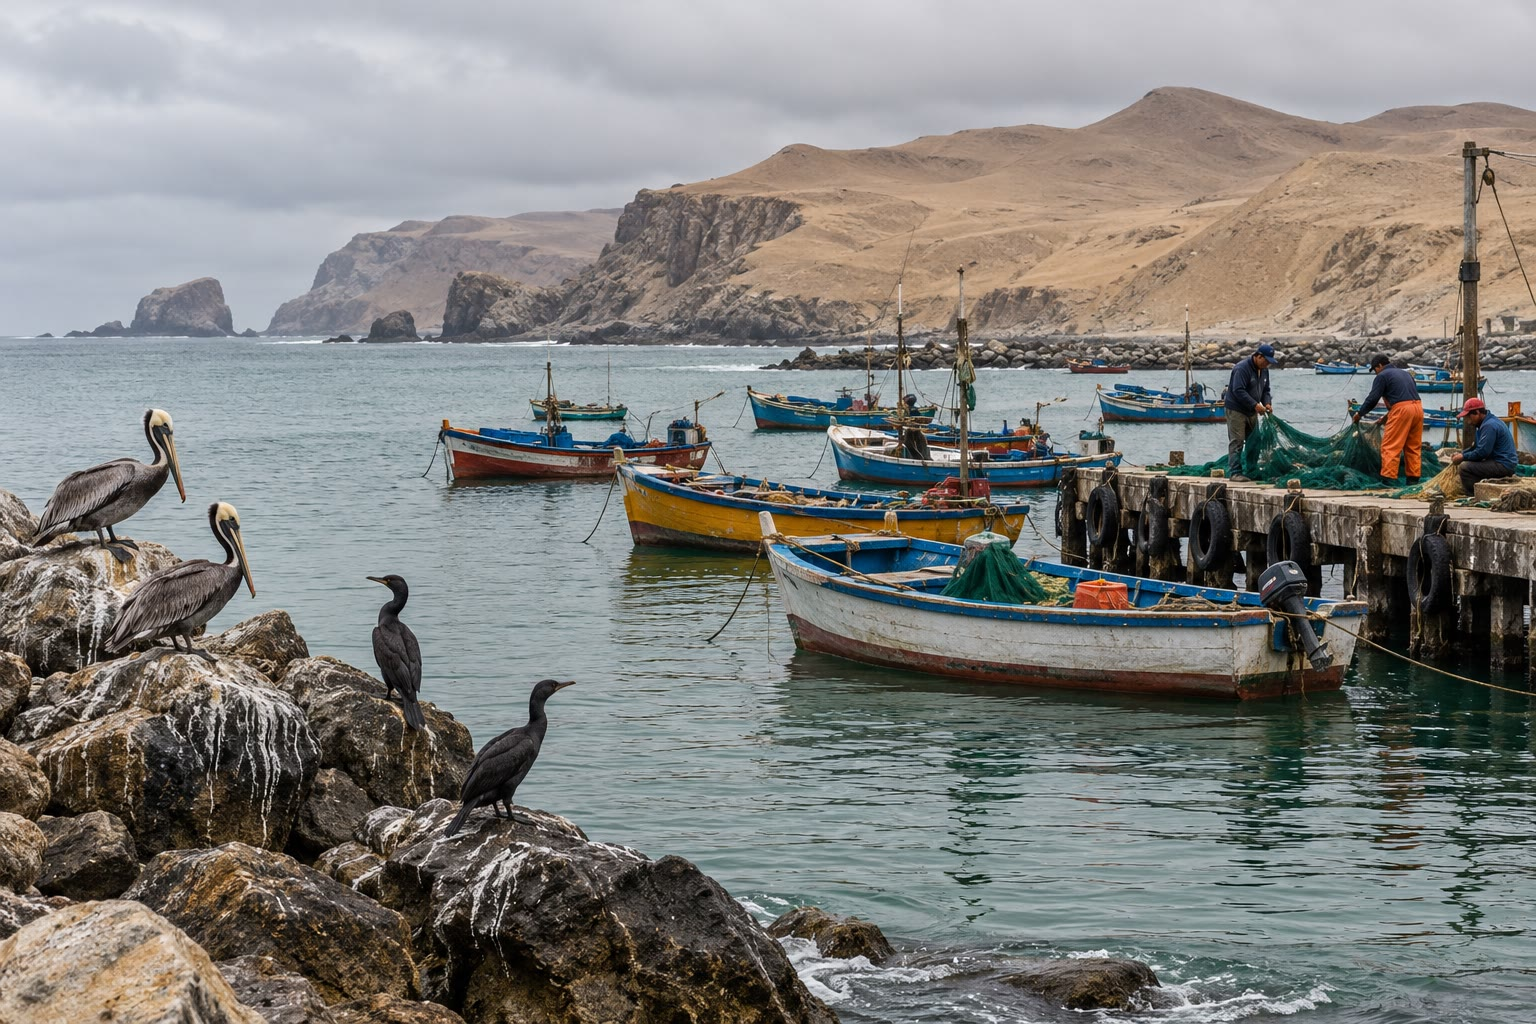
\includegraphics[width=\linewidth]{images/book4/ai/b2-fishing-harbour.jpg}

{\scriptsize Barcos de pesca num porto de uma costa desértica com água fria de ressurgência
(ilustração gerada por IA).}
\end{minipage}
% ledger: climategov:enso-history, cheung26:peru, stewart:upwelling
\end{history}

Por que o sistema oscila? Porque o oceano e a atmosfera do Pacífico equatorial
reforçam as anomalias um do outro.

\begin{definition}[Retroalimentação de Bjerknes]\label{def:b2:climate-variability:bjerknes}
A \emph{retroalimentação de Bjerknes}\index{retroalimentação de Bjerknes} é a retroalimentação positiva entre a
temperatura da superfície do mar, os ventos e as correntes oceânicas do Pacífico equatorial: um aquecimento do
leste enfraquece o contraste leste--oeste de temperatura e de pressão, e portanto os alísios;
alísios mais fracos deixam a água quente do oeste espalhar-se para leste e fazem subir menos água fria no
leste, o que aquece ainda mais o leste. O mesmo circuito amplifica um resfriamento.
\end{definition}
% ledger: thirumalai24:bjerknes, cpc:enso-faq-timing

\begin{omfigure}
\centering
\begin{tikzpicture}[font=\small, >=Stealth, box/.style={draw, rounded corners=2pt, fill=omDef!8,
  align=center, text width=4.3cm, minimum height=1.05cm, inner sep=3pt}]
\node[box] (a) at (0,2) {Pacífico equatorial oriental\\mais quente que o habitual};
\node[box] (b) at (6.2,2) {menor contraste leste--oeste\\de temperatura e pressão};
\node[box] (c) at (6.2,0) {alísios mais fracos};
\node[box] (d) at (0,0) {água quente para leste,\\sobe menos água fria};
\draw[->, very thick, ocRed] (a) -- (b);
\draw[->, very thick, ocRed] (b) -- (c);
\draw[->, very thick, ocRed] (c) -- (d);
\draw[->, very thick, ocRed] (d) -- (a);
\node[ocRed, font=\bfseries] at (3.1,1) {$+$};
\end{tikzpicture}
\par\smallskip{\small A \omterm{def:b2:climate-variability:bjerknes}{retroalimentação de Bjerknes}, desenhada para um aquecimento; com todas as setas invertidas, o
mesmo circuito aprofunda um resfriamento. Um circuito positivo desse tipo amplifica uma pequena perturbação.}
\end{omfigure}
% ledger: thirumalai24:bjerknes

Uma retroalimentação positiva explica como uma anomalia cresce, não como começa nem como termina. Segundo uma explicação atual,
um El~Niño começa quando flutuações aleatórias dos alísios enfraquecem as correntes equatoriais que
mantêm a água quente no oeste; a piscina quente espalha-se para leste, a convecção a acompanha, a
\omterm{def:b2:climate-variability:bjerknes}{retroalimentação de Bjerknes} assume o controle e o evento cresce. Os eventos La~Niña, na mesma explicação, são
desencadeados por um El~Niño anterior. Os modelos mais simples que fazem o sistema oscilar, entre eles o
oscilador de recarga, acoplam duas grandezas: a anomalia de temperatura da superfície do mar do Pacífico
central e o volume de água quente da camada superior do oceano armazenado ao longo do equador. A anomalia
de temperatura esvazia ou reabastece esse estoque através dos ventos que provoca, e o estoque, através da
profundidade da termoclina, prepara a fase seguinte. O \cref{exo:b2:climate-variability:10} resolve
um tal par de equações.
% ledger: thirumalai24:bjerknes, stuecker25:ro

Para acompanhar o ENSO, os centros de monitoramento usam índices.

\begin{definition}[Índice Niño-3.4; Índice Oceânico Niño]\label{def:b2:climate-variability:oni}
O \emph{índice Niño-3.4}\index{índice Niño-3.4} é a anomalia mensal da temperatura da superfície
do mar média sobre a região \ang{5} N--\ang{5} S, \ang{170} W--\ang{120} W, em relação à
\omterm{def:b2:climate-variability:modes}{climatologia} de um período de base de 30 anos centrado no ano, atualizado a cada cinco anos. O
\emph{Índice Oceânico Niño}\index{Índice Oceânico Niño} (ONI) é sua média móvel de três meses. Um
episódio de El~Niño (de La~Niña) é uma sequência de pelo menos cinco estações de três meses consecutivas e sobrepostas
com o ONI igual ou superior a \qty{+0.5}{\celsius} (igual ou inferior a \qty{-0.5}{\celsius}).
\end{definition}
% ledger: cpc:oni-def, cpc:enso-faq

As estações sobrepõem-se: DJF, JFM, FMA e assim por diante, cada uma a média de três meses, cada uma com dois
meses em comum com a seguinte. Um segundo índice, o Índice de \omterm{def:b2:climate-variability:enso}{Oscilação Sul}, acompanha a atmosfera: ele
é calculado a partir dos desvios da diferença de pressão entre o Taiti e Darwin, negativo
durante o El~Niño, positivo durante a La~Niña. Desde fevereiro de 2026 o índice oficial de monitoramento do
ENSO é um ONI relativo, calculado a partir da anomalia Niño-3.4 menos a anomalia média de todo o
oceano tropical entre \ang{20} N e \ang{20} S, depois reescalonado para a amplitude do ONI. Por ser
medido em relação aos trópicos inteiros, ele depende menos da escolha do período de base enquanto os oceanos
aquecem, e relaciona-se melhor com a chuva do Pacífico tropical. Em setembro de 2026 a
anomalia relativa da região Niño-3.4 era de \qty{2.08}{\celsius}, contra os \qty{2.56}{\celsius}
do \cref{ex:b2:climate-variability:anomaly}: cerca de meio grau da anomalia tradicional era o
calor dos oceanos tropicais como um todo.
% ledger: cpc:enso-faq-so, pns:roni, data:b4-rnino34

\begin{omfigure}
\centering
% figdata/bachelor-2/climvar.py part oni
\begin{tikzpicture}
\begin{axis}[width=\linewidth, height=6.0cm, xmin=1950, xmax=2027, ymin=-2.4, ymax=3.0,
  xlabel={ano}, ylabel={índice (\unit{\celsius})}, tick label style={font=\scriptsize},
  label style={font=\small}, xtick={1950,1960,...,2020}, x tick label style={/pgf/number
  format/1000 sep={}}, legend style={font=\scriptsize, at={(0.5,1.02)}, anchor=south,
  draw=none, legend columns=3, /tikz/every even column/.append style={column sep=6pt}},
  legend cell align=left]
\addplot[fill=ocRed!70, draw=none, area legend] table[x=t, y=pos]
  {figdata/out/bachelor-2-climvar-oni.dat} \closedcycle;
\addlegendentry{ONI, lado El Niño}
\addplot[fill=ocBlue!70, draw=none, area legend] table[x=t, y=neg]
  {figdata/out/bachelor-2-climvar-oni.dat} \closedcycle;
\addlegendentry{ONI, lado La Niña}
\addplot[black, thin] table[x=t, y=roni] {figdata/out/bachelor-2-climvar-oni.dat};
\addlegendentry{ONI relativo}
\addplot[black!60, densely dashed, domain=1950:2027, samples=2] {0.5};
\addplot[black!60, densely dashed, domain=1950:2027, samples=2] {-0.5};
\end{axis}
\end{tikzpicture}
\par\smallskip{\small O \omterm{def:b2:climate-variability:oni}{Índice Oceânico Niño} de DJF de 1950 a JAS de 2026 (um valor por
estação de três meses, situado em seu mês central), e o ONI relativo, índice oficial desde
fevereiro de 2026; tracejado: os limiares $\pm\qty{0.5}{\celsius}$. Dados: NOAA Climate Prediction
Center, obtidos em 23 de outubro de 2026.}
\end{omfigure}
% ledger: data:b4-oni, data:b4-roni

Contados com a regra das cinco estações na tabela do Climate Prediction Center, o ONI mostra 25
episódios de El~Niño e 21 de La~Niña entre 1950 e o verão (boreal) de 2026. Os picos mais fortes de El~Niño
foram \qty{2.4}{\celsius} no fim de 1997 e \qty{2.6}{\celsius} no fim de 2015. Os dois índices
divergem mais nos anos recentes: em julho--setembro de 2026 o ONI estava em \qty{2.2}{\celsius} e
o índice relativo em \qty{1.7}{\celsius}.
% ledger: data:b4-oni, data:b4-roni

\begin{dated}{2026}
Em sua discussão de 8 de outubro de 2026 o Climate Prediction Center manteve seu alerta de El~Niño: a
anomalia relativa Niño-3.4 tinha atingido \qty{+2.1}{\celsius} em setembro, partes do Pacífico
equatorial oriental estavam mais de \qty{4}{\celsius} acima da média, a água em profundidade no leste
mais de \qty{10}{\celsius} acima, e os índices da \omterm{def:b2:climate-variability:enso}{Oscilação Sul} estavam significativamente
negativos. Um
El~Niño de forte a muito forte foi julgado provável até janeiro--março de 2027, e a probabilidade de
o índice relativo ultrapassar \qty{2.5}{\celsius}, além de todos os eventos desde 1950, foi estimada em
\qty{83}{\percent} para outubro--dezembro.
% ledger: cpc:edd-2026-10, data:b4-rnino34
\end{dated}

\section{A Oscilação do Atlântico Norte e as teleconexões}\label{sec:b2:climate-variability:nao}

\begin{definition}[Oscilação do Atlântico Norte]\label{def:b2:climate-variability:nao}
A \emph{Oscilação do Atlântico Norte}\index{Oscilação do Atlântico Norte} (NAO) é o modo dominante
de variabilidade atmosférica sobre o Atlântico Norte: uma gangorra de pressão ao nível do mar entre a
Baixa da Islândia e a Alta dos Açores. Seu índice é positivo quando ambas estão mais fortes que a média, de modo
que a diferença de pressão entre elas é grande, e negativo quando ambas estão mais fracas.
\end{definition}
% ledger: ipccgl:other-modes, climategov:nao, cpc:nao-teledoc

A NAO dirige os ventos de oeste do capítulo anterior. Em sua fase positiva a maior diferença de
pressão move uma corrente de jato atlântica mais forte e desloca a trajetória das tempestades para o norte: o norte da Europa
tem um inverno mais tempestuoso, mais úmido e mais ameno, o sul da Europa um inverno mais seco, o leste da América do Norte
menos irrupções de ar frio, e a Groenlândia um inverno mais frio. A fase negativa inverte essas
anomalias. No fim do século XVIII um missionário já notava que os invernos amenos na
Groenlândia vinham com invernos rigorosos na Dinamarca, e o inverso.
% ledger: climategov:nao, cpc:nao-teledoc

A NAO é um dos padrões mais marcantes da atmosfera em todas as estações, e está
fortemente correlacionada com outro modo, a Oscilação Ártica. Também varia ao longo de décadas: a fase negativa dominou
de meados dos anos 1950 ao inverno de 1978--79, e a fase positiva de 1979--80 a 1994--95.
% ledger: cpc:nao-teledoc, climategov:nao

\begin{omfigure}
\centering
% figdata/bachelor-2/climvar.py part nao
\begin{tikzpicture}
\begin{axis}[width=\linewidth, height=5.4cm, xmin=1950, xmax=2027, ymin=-1.9, ymax=1.9,
  ytick={-1,0,1},
  xlabel={inverno (ano de seu janeiro)}, ylabel={índice NAO (média DJF)},
  tick label style={font=\scriptsize}, label style={font=\small}, xtick={1950,1960,...,2020},
  x tick label style={/pgf/number format/1000 sep={}}, legend style={font=\scriptsize,
  at={(0.5,1.02)}, anchor=south, draw=none, legend columns=2,
  /tikz/every even column/.append style={column sep=6pt}},
  legend cell align=left, unbounded coords=jump]
\addplot[ybar, bar width=0.6, fill=omDef!55, draw=none, area legend] table[x=year, y=nao]
  {figdata/out/bachelor-2-climvar-nao.dat};
\addlegendentry{média de inverno}
\addplot[ocRed, thick] table[x=year, y=run5] {figdata/out/bachelor-2-climvar-nao.dat};
\addlegendentry{média móvel de 5 invernos}
\end{axis}
\end{tikzpicture}
\par\smallskip{\small A média de inverno (dezembro--fevereiro) do índice NAO mensal do NOAA
Climate Prediction Center, 1951--2026, em desvios-padrão, com sua média móvel centrada de cinco
invernos. O inverno mais baixo é o de 2010 ($-1.67$), o mais alto o de 2015 ($+1.66$).}
\end{omfigure}
% ledger: data:b4-nao, cpc:nao-teledoc

A NAO, o ENSO e os outros modos agem longe de onde são medidos.

\begin{definition}[Teleconexão]\label{def:b2:climate-variability:teleconnection}
Uma \emph{teleconexão}\index{teleconexão} é uma associação entre variáveis climáticas em
lugares fixos e muito afastados, ligados por processos físicos ao longo de caminhos na atmosfera ou no
oceano, como trens de \omterm{def:b2:weather-systems:rossby}{ondas de Rossby}, deslocamentos da corrente de jato e das trajetórias das tempestades, ou mudanças
da circulação de Walker.
\end{definition}
% ledger: ipccgl:teleconnection

Durante o El~Niño a chuva dos trópicos muda da Indonésia à América do Sul, cerca de meia
volta ao mundo, e a partir dos trópicos as anomalias viajam até as latitudes médias pelos caminhos
da definição; a \omterm{def:b2:climate-variability:monsoon}{monção} indiana da seção anterior é uma de suas extremidades. Outros modos
receberam nomes em cada oceano: o Dipolo do Oceano Índico, uma gangorra leste--oeste da temperatura da superfície
do mar no oceano Índico tropical, cuja fase positiva esfria o mar ao largo de Sumatra e de Java
e aquece-o ao largo da Somália, que se desenvolve no verão boreal, amadurece no outono e muda
a chuva da Austrália, do Sudeste Asiático e da África Oriental; o Modo Anular Sul, as mudanças de
intensidade e de latitude do cinturão de ventos de oeste em volta da Antártida; e a variabilidade decenal do
Pacífico, mais lenta que o ENSO.
% ledger: cpc:enso-faq, ipccgl:other-modes, ipccgl:teleconnection, narang24:enso-monsoon

\section{O oceano como memória}\label{sec:b2:climate-variability:memory}

O \cref{ch:b2:weather-systems} concluiu que a atmosfera esquece seu tempo em cerca de duas semanas.
Uma anomalia climática que dura uma estação tem de ser armazenada em algum lugar, e o reservatório óbvio é a camada
de mistura do oceano: uma camada de mistura mais profunda guarda mais calor e tem mais inércia térmica. O modelo mais simples trata a
anomalia como um reservatório que perde calor para a atmosfera.
% ledger: shi22:memory

\begin{proposition}[Tempo de amortecimento de uma anomalia da camada de mistura]\label{prop:b2:climate-variability:damping}
Suponha-se que uma camada de mistura de profundidade $h$, densidade $\rho$ e calor específico $c_p$ tenha uma anomalia de temperatura
$T'$, e que a superfície perca um fluxo de calor suplementar $\alpha T'$ por unidade de área para a atmosfera,
com $\alpha > 0$. Então, sem outro forçamento,
\[
  T'(t) = T'(0)\,\mathrm{e}^{-t/\tau}, \qquad \tau = \frac{\rho\,c_p\,h}{\alpha} .
\]
\end{proposition}

\begin{proof}
O conteúdo de calor da anomalia por unidade de área é $\rho c_p h T'$; o primeiro princípio dá $\rho c_p h
\,\mathrm{d}T'/\mathrm{d}t = -\alpha T'$, uma equação linear cuja solução é o decaimento
exponencial com a constante de tempo $\tau$.
\end{proof}
% ledger: shi22:memory

\begin{example}[A memória de um oceano de latitudes médias]\label{ex:b2:climate-variability:tau}
Sobre os oceanos das latitudes médias, o fluxo de calor à superfície responde a uma anomalia de temperatura da superfície
do mar com um valor médio $\alpha = \qty{16.1}{W.m^{-2}.K^{-1}}$. Para uma camada de mistura
de \qty{50}{m} de profundidade, com $\rho = \qty{1025}{kg/m^3}$ e $c_p = \qty{3992}{J.kg^{-1}.K^{-1}}$,
$\tau = 1025 \times 3992 \times 50/16.1 = \qty{1.27e7}{s} = \qty{147}{\day}$, quase cinco
meses; uma camada de \qty{100}{m} de profundidade lembra-se durante o dobro do tempo.
\end{example}
% ledger: wang24:shff, noaa:seawater-1025, teos10:cp0

As anomalias reais também são forçadas, todos os dias, pelo tempo: fluxos aleatórios de calor que, sozinhos,
produziriam um ruído branco, sem memória de um mês para o outro. Somados ao amortecimento, eles
dão a equação $\mathrm{d}T'/\mathrm{d}t = -T'/\tau + F(t)$ com um $F$ aleatório: o oceano soma
o forçamento aleatório ao longo de um tempo da ordem de $\tau$ e esquece-o além disso. O resultado chama-se
ruído vermelho. Sua correlação defasada, a correlação entre a anomalia e ela mesma algum tempo depois,
cai como $\mathrm{e}^{-\text{defasagem}/\tau}$ (admitido), e as variações lentas são muito mais fortes nele
do que no forçamento. Esse modelo estocástico da memória do oceano é a referência padrão
com a qual se mede a persistência das anomalias reais, uma fonte de previsibilidade além
das escalas de tempo do tempo meteorológico; como a profundidade da camada de mistura fixa a memória, a diminuição da profundidade das
camadas de mistura projetada para este século implica uma memória mais curta.
% ledger: shi22:memory

\begin{omfigure}
\centering
% figdata/bachelor-2/climvar.py parts rednoise, acf
\begin{tikzpicture}
\begin{groupplot}[group style={group size=2 by 1, horizontal sep=1.6cm},
  tick label style={font=\scriptsize}, label style={font=\small}]
\nextgroupplot[width=0.62\linewidth, height=5.0cm, xmin=0, xmax=360, ymin=-1.6, ymax=1.6,
  xlabel={mês}, ylabel={anomalia (\unit{K})}, xtick={0,60,...,360},
  legend style={font=\scriptsize, at={(0.5,1.02)}, anchor=south, draw=none, legend columns=2},
  legend cell align=left]
\addplot[black!45, thin] table[x=month, y=white] {figdata/out/bachelor-2-climvar-rednoise.dat};
\addlegendentry{ruído branco}
\addplot[ocRed, thick] table[x=month, y=red] {figdata/out/bachelor-2-climvar-rednoise.dat};
\addlegendentry{ruído vermelho, $\tau = \qty{147}{\day}$}
\nextgroupplot[width=0.36\linewidth, height=5.0cm, xmin=0, xmax=24, ymin=0, ymax=1.05,
  xlabel={defasagem (meses)}, ylabel={correlação defasada}, xtick={0,6,...,24},
  legend style={font=\scriptsize, at={(0.98,0.98)}, anchor=north east, draw=none},
  legend cell align=left]
\addplot[black, densely dashed] table[x=lag_months, y=theory] {figdata/out/bachelor-2-climvar-acf.dat};
\addlegendentry{$\mathrm{e}^{-\text{defasagem}/\tau}$}
\addplot[only marks, mark=*, mark size=1.1pt, ocRed] table[x=lag_months, y=sample]
  {figdata/out/bachelor-2-climvar-acf.dat};
\addlegendentry{simulada}
\end{groupplot}
\end{tikzpicture}
\par\smallskip{\small Um ruído vermelho e um ruído branco de mesmo desvio-padrão, 0.5~K, em
médias mensais ao longo de 30 anos (esquerda): a camada de mistura do
\cref{ex:b2:climate-variability:tau} transforma um forçamento diário aleatório em oscilações lentas. Direita: a
correlação defasada de uma simulação de 2000 anos contra $\mathrm{e}^{-\text{defasagem}/\tau}$.}
\end{omfigure}
% ledger: shi22:memory, wang24:shff

O ENSO precisa de mais do que essa memória passiva. Suas anomalias envolvem não só a camada de mistura, mas
toda a camada quente acima da termoclina, que se desloca dezenas de metros, e os ventos que as
anomalias provocam retroagem sobre o oceano pelo circuito de Bjerknes. O oceano fornece a lentidão,
a atmosfera o acoplamento; nenhum dos dois sozinho produz a oscilação. A lentidão é aquilo em que se apoiaram os
previsores de outubro de 2026 quando julgaram provável que um forte El~Niño durasse até
janeiro--março de 2027.
% ledger: cpc:enso-faq-features, cpc:enso-faq-timing, climategov:enso-history, cpc:edd-2026-10

\section*{Exercícios}\label{sec:b2:climate-variability:exercises}

Dados para os exercícios, salvo indicação em contrário: água do mar $\rho = \qty{1025}{kg/m^3}$ e $c_p =
\qty{3992}{J.kg^{-1}.K^{-1}}$; ar $c_p = \qty{1004.5}{J.kg^{-1}.K^{-1}}$; $g =
\qty{9.81}{m.s^{-2}}$; o coeficiente de amortecimento do fluxo de calor à superfície $\alpha =
\qty{16.1}{W.m^{-2}.K^{-1}}$; um mês tem $365.25/12 = 30.44$ dias.
% ledger: noaa:seawater-1025, teos10:cp0, wang24:shff

\begin{exercise}[$\star$]\label{exo:b2:climate-variability:1}
Na região Niño-3.4 a temperatura média da superfície do mar foi de \qty{29.27}{\celsius} em setembro de
2026 e de \qty{28.79}{\celsius} em setembro de 1997; as \omterm{def:b2:climate-variability:modes}{climatologias} usadas para esses dois meses de setembro
foram \qty{26.71}{\celsius} e \qty{26.73}{\celsius}. (a) Calcule as duas anomalias. (b) Qual
setembro foi mais quente, e qual anomalia foi maior? (c) Por que a \omterm{def:b2:climate-variability:modes}{climatologia} não é a mesma para os
dois anos?
\end{exercise}
% ledger: data:b4-nino34, cpc:oni-def

\begin{exercise}[$\star$]\label{exo:b2:climate-variability:2}
As anomalias mensais Niño-3.4 de junho a dezembro de 2023 foram 0.79, 0.95, 1.28, 1.55, 1.68, 2.01
e \qty{2.02}{\celsius}. (a) Calcule o ONI das estações JJA a OND. (b) A tabela do
Climate Prediction Center dá 1.0, 1.3, 1.5, 1.7 e 1.9. Compare. (c) Em que estação o
ONI atingiu pela primeira vez o limiar de um evento forte, \qty{1.5}{\celsius}?
\end{exercise}
% ledger: data:b4-nino34-2023, data:b4-oni-cases

\begin{exercise}[$\star$]\label{exo:b2:climate-variability:3}
Num certo mês a pressão à superfície está acima da média em Darwin e abaixo da média no Taiti.
(a) Qual é o sinal do Índice de \omterm{def:b2:climate-variability:enso}{Oscilação Sul}? (b) Que fase do ENSO ele sugere?
(c) O que você espera para os alísios sobre o Pacífico equatorial oriental, e para a
chuva sobre a Indonésia?
\end{exercise}
% ledger: cpc:enso-faq-so, cpc:enso-faq-features

\begin{exercise}[$\star$]\label{exo:b2:climate-variability:4}
(a) A chuva de junho a setembro de 2018 sobre a Índia foi de \qty{804.1}{mm}, contra uma
média de longo período de \qty{880.6}{mm}. Calcule-a em porcentagem da média e classifique
a estação. (b) Na costa de Kerala as médias de junho, julho, agosto e setembro são 556,
659, 427 e \qty{252}{mm}. Que fração da chuva da estação cai em julho?
\end{exercise}
% ledger: imd:lpa

\begin{exercise}[$\star\star$]\label{exo:b2:climate-variability:5}
(a) Calcule o tempo de amortecimento de uma anomalia em camadas de mistura de \qty{50}{m} e de \qty{100}{m} de profundidade.
(b) Calcule, para cada uma, a correlação defasada da anomalia após um mês. (c) Os modelos climáticos
projetam camadas de mistura mais rasas num clima mais quente. O que isso faz com a memória do
oceano?
\end{exercise}
% ledger: wang24:shff, shi22:memory

\begin{exercise}[$\star\star$]\label{exo:b2:climate-variability:6}
Observa-se uma anomalia de temperatura da superfície do mar de \qty{+1.2}{K} sobre uma camada de mistura de \qty{50}{m}
de profundidade. (a) Sem forçamento adicional, que anomalia resta após três meses, e após seis? (b)
Uma tal previsão, que apenas deixa a anomalia presente decair, chama-se previsão por persistência.
Por que é melhor do que supor nenhuma anomalia, e por que piora com o tempo?
\end{exercise}

\begin{exercise}[$\star\star$]\label{exo:b2:climate-variability:7}
Em junho o solo dos desertos do noroeste da Índia e do Paquistão envia cerca de
\qty{160}{W/m^2} de calor para o ar. (a) Quanta energia é isso por metro quadrado e por dia?
(b) Se ela ficasse toda na camada entre o solo a \qty{1000}{hPa} e \qty{850}{hPa}, a que
ritmo essa camada aqueceria? (c) Na realidade a baixa térmica não aquece a esse ritmo semana após semana.
Cite duas maneiras pelas quais o calor pode sair da camada.
\end{exercise}
% ledger: imd:heat-low

\begin{exercise}[$\star\star$]\label{exo:b2:climate-variability:8}
O índice NAO mensal foi de $-1.93$ em dezembro de 2009, $-1.11$ em janeiro de 2010 e $-1.98$ em
fevereiro de 2010. (a) Calcule a média do inverno. (b) Em 1951--2026 as médias de inverno vão de
$-1.67$ a $+1.66$. Situe este inverno. (c) Que tempo de inverno você esperaria no norte da
Europa, no sul da Europa e no leste dos Estados Unidos?
\end{exercise}
% ledger: data:b4-nao, climategov:nao

\begin{exercise}[$\star\star$]\label{exo:b2:climate-variability:9}
Uma região pertence ao domínio global das \omterm{def:b2:climate-variability:monsoon}{monções} quando a chuva média de seu verão local excede a
de seu inverno em mais de \qty{2.5}{mm} por dia. (a) Uma estação inventada do Hemisfério
Norte recebe em média \qty{9.3}{mm} por dia em junho--agosto e \qty{0.4}{mm} por dia em
dezembro--fevereiro. Está no domínio? (b) Uma estação inventada do Hemisfério Sul
recebe \qty{4.2}{mm} por dia em junho--agosto e \qty{6.1}{mm} por dia em dezembro--fevereiro. E
ela? (c) Na costa de Kerala a chuva média de junho a setembro (122 dias) é de 556, 659, 427 e
\qty{252}{mm} mês a mês. Calcule sua taxa diária média, e a taxa de inverno acima da qual Kerala,
tomando junho--setembro como seu verão, ficaria fora do domínio. (d) Por que o critério
usa a diferença entre as estações e não a chuva total do ano?
\end{exercise}
% ledger: ipccgl:monsoon, imd:lpa

\begin{exercise}[$\star\star\star$]\label{exo:b2:climate-variability:10}
Um oscilador de recarga simples escreve a anomalia de temperatura Niño-3.4 $T$ e a anomalia $H$ da
água quente armazenada ao longo do equador como $\dot T = aH$, $\dot H = -bT$, com $a, b > 0$. (a) Mostre
que $T$ oscila, com o período $2\pi/\sqrt{ab}$. (b) Que produto $ab$ dá um período de
quatro anos? (c) Com amortecimento, $\dot T = aH - rT$ e $\dot H = -bT - rH$, mostre que
$(T\,\mathrm{e}^{rt}, H\,\mathrm{e}^{rt})$ obedece às equações sem amortecimento. Com $r = 0.25$ por
ano, por que fator a amplitude diminui num período? (d) O que deve manter a
oscilação real?
\end{exercise}
% ledger: stuecker25:ro, thirumalai24:bjerknes, ipccgl:enso

\begin{exercise}[$\star\star\star$]\label{exo:b2:climate-variability:11}
A região Niño-3.4 estende-se por \ang{10} em latitude e \ang{50} em longitude ao longo do equador
(tome um raio terrestre de \qty{6371}{km}). (a) Calcule sua área. (b) Quanto calor é preciso para
aquecer em \qty{2}{K} uma camada de \qty{100}{m} de profundidade sobre essa área? (c) Que fluxo de calor suplementar à superfície,
mantido durante seis meses, o forneceria? (d) Durante o El~Niño os alísios enfraquecem e a
termoclina no leste aprofunda-se. De onde mais pode vir o calor?
\end{exercise}
% ledger: cpc:oni-def, cpc:enso-faq-features

\begin{exercise}[$\star\star\star$]\label{exo:b2:climate-variability:12}
Trate a \omterm{def:b2:climate-variability:bjerknes}{retroalimentação de Bjerknes} como um circuito que devolve, como aquecimento suplementar, uma fração $g$ de todo
aquecimento que passa por ele. (a) Uma rajada de vento de oeste aquece o leste em \qty{0.3}{K}. Mostre
que o aquecimento total é $0.3/(1 - g)$, e calcule-o para $g = 0.5$, 0.8 e 0.9. (b) O que
acontece se $g \geq 1$, e o que deve então limitar o evento? (c) Por que $g$ deveria ser máximo na
estação em que o Pacífico equatorial está mais quente?
\end{exercise}
% ledger: thirumalai24:bjerknes, cpc:enso-faq-timing

\begin{problem}[{Problema de fim de semana --- contar os El Niño}]\label{pb:b2:climate-variability:1}
Das temperaturas mensais do mar ao registro do El~Niño desde 1950, e ao oceano que o torna
possível. Use os dados dos exercícios.

\medskip\noindent\textbf{Parte I --- Dos meses às estações.}
As anomalias mensais Niño-3.4 de abril de 1997 a janeiro de 1998 foram 0.26, 0.75, 1.13, 1.52, 1.80,
2.06, 2.26, 2.42, 2.36 e \qty{2.33}{\celsius}.
\begin{enumerate}
  \item Calcule o ONI da estação AMJ de 1997.
  \item Calcule o ONI de MJJ, JJA e JAS.
  \item Calcule o ONI de ASO, SON, OND e NDJ.
  \item A tabela do Climate Prediction Center dá 0.7, 1.1, 1.5, 1.8, 2.0, 2.2, 2.3 e
        2.4 para essas oito estações. Compare.
  \item Por que o índice faz a média de três meses em vez de usar meses isolados?
  \item Em que estação o evento de 1997 se tornou forte ($\geq \qty{1.5}{\celsius}$), e em
        que valor atingiu o pico?
\end{enumerate}

\medskip\noindent\textbf{Parte II --- A regra das cinco estações.}
O ONI do Climate Prediction Center para 2018 a 2020 é, estação por estação, de DJF a
NDJ: 2018: $-0.7$, $-0.7$, $-0.5$, $-0.3$, $-0.1$, 0.1, 0.2, 0.3, 0.5, 0.8, 1.0, 1.1; 2019: 1.0,
0.9, 0.9, 0.8, 0.7, 0.6, 0.4, 0.2, 0.3, 0.5, 0.7, 0.8; 2020: 0.7, 0.7, 0.6, 0.3, 0.0, $-0.2$,
$-0.3$, $-0.4$, $-0.8$, $-1.0$, $-1.1$, $-1.1$; depois DJF de 2021 $-1.0$ e JFM de 2021 $-0.9$. O
ONI relativo é, a partir de SON de 2018: 0.62, 0.82, 0.78; 2019: 0.68, 0.64, 0.57, 0.53, 0.37, 0.24,
0.04, $-0.12$, $-0.01$, 0.15, 0.29, 0.22; 2020: 0.14, 0.10, 0.02, $-0.25$, $-0.55$, $-0.72$,
$-0.76$, $-0.85$, $-1.16$, $-1.37$, $-1.46$, $-1.39$.
\begin{enumerate}[resume]
  \item Encontre os episódios de El~Niño de 2018--2020 segundo o ONI: primeira e última estação de cada um.
  \item Quantas estações dura cada um?
  \item Em que estação começa a La~Niña seguinte segundo o ONI, e por que você precisa dos
        valores de 2021 para ter certeza?
  \item Encontre os episódios de El~Niño segundo o ONI relativo, e a primeira estação da La~Niña.
  \item O evento do fim de 2019 é um El~Niño segundo o ONI relativo? Explique a diferença
        entre os dois índices em 2019.
\end{enumerate}

\medskip\noindent\textbf{Parte III --- Os El Niño fortes.}
Os episódios de El~Niño desde 1950 cujo ONI de pico atingiu pelo menos \qty{1.5}{\celsius} começaram nas
estações MAM de 1957, AMJ de 1965, AMJ de 1972, AMJ de 1982, JAS de 1986, AMJ de 1991, AMJ de 1997, JJA de 2009, SON de 2014,
AMJ de 2023 e MAM de 2026, com picos de 1.7, 1.8, 1.8, 2.1, 1.5, 1.5, 2.4, 1.5, 2.6, 2.0 e, em
JAS de 2026, \qty{2.2}{\celsius} e subindo. Conte em anos, a partir do ano em que cada um começou.
\begin{enumerate}[resume]
  \item Quantos episódios fortes há?
  \item Liste os intervalos entre os inícios de episódios fortes sucessivos.
  \item Qual intervalo é o mais curto, qual o mais longo?
  \item Calcule o intervalo médio de duas maneiras: como a média dos intervalos, e como o tempo
        do primeiro início ao último dividido pelo número de intervalos. Por que concordam?
  \item O evento de 2026 ainda estava crescendo quando os dados terminam. Por que ele conta mesmo assim
        como episódio forte, e por que nenhum dado posterior pode mudar seu início?
  \item As perguntas frequentes do Climate Prediction Center dizem que o El~Niño e a La~Niña ocorrem a cada 3 a 5
        anos. O intervalo médio dos fortes é compatível com isso?
\end{enumerate}

\medskip\noindent\textbf{Parte IV --- Por que o ENSO precisa do oceano.}
Tome uma camada de mistura de \qty{50}{m} de profundidade e uma coluna de ar de \qty{1000}{hPa}.
\begin{enumerate}[resume]
  \item Calcule o tempo de amortecimento de uma anomalia da camada de mistura.
  \item Calcule a capacidade térmica por metro quadrado da camada de mistura e da coluna de ar
        inteira acima dela.
  \item Que profundidade de água do mar tem a capacidade térmica de toda a atmosfera acima dela?
  \item Calcule o tempo de amortecimento de uma anomalia carregada só pela coluna de ar, com o mesmo
        $\alpha$.
  \item Por que o oceano consegue levar uma anomalia do ENSO de uma estação para a seguinte, e a
        atmosfera não?
  \item Em resumo: quantos anos, em média, separam os inícios de episódios fortes sucessivos de El~Niño
        desde 1950?
\end{enumerate}
\end{problem}
% ledger: data:b4-nino34, data:b4-oni, data:b4-oni-cases, data:b4-roni-cases, cpc:enso-faq-timing, wang24:shff
